% !TEX root = omar-thesis-proposal.tex
\newcommand{\atlam}{@$\lambda$}

% Generic
\newcommand{\bindin}[2]{#1;~#2}
\newcommand{\pipe}{~\text{\large $\vert$}~}
\newcommand{\splat}[3]{#1_{#2};\ldots;#1_{#3}}
\newcommand{\splatC}[3]{#1_{#2}~~~~\cdots~~~~#1_{#3}}
\newcommand{\splatTwo}[4]{#1_{#3}#2_{#3},~\ldots~, #1_{#4}#2_{#4}}
\newcommand{\substn}[2]{[#1]#2}
\newcommand{\subst}[3]{\substn{#1/#2}{#3}}
\newcommand{\entails}[2]{#1 \vdash #2}

% Programs
\newcommand{\progsort}{\rho}
\newcommand{\pfam}[2]{\bindin{#1}{#2}}
\newcommand{\pdef}[4]{\bindin{{\sf def}~\tvar{#1}:#2=#3}{#4}}

% Families
\newcommand{\fvar}[1]{\textsc{#1}}

\newcommand{\family}[6]{{\sf family}~\fvar{#1}[#2]\sim \tvar{#5}.#6~\{#3\}}
\newcommand{\familyDf}{\family{Fam}{\kappaidx}{\opsort}{\opsigsort}{i}{\taurep}}

% Operators
\newcommand{\opsort}{\theta}
\newcommand{\opsigsort}{\Theta}
\newcommand{\opvar}[1]{\textbf{\textit{#1}}}

% Expressions
\newcommand{\evar}[1]{#1}
\newcommand{\elam}[3]{\lambda #1{:}#2.#3}
\newcommand{\eapp}[2]{{#1~#2}}
\newcommand{\eopapp}[2]{\eop{Arrow}{ap}{\tunit}{#1; #2}}
\newcommand{\eop}[4]{{\fvar{#1}.\opvar{#2}\langle#3\rangle(#4)}}
\newcommand{\elet}[4]{{\sf let}~#1 : #2 = #3~{\sf in}~#4}

% Type-Level Terms
\newcommand{\tvar}[1]{{\textbf{#1}}}

\newcommand{\tlam}[3]{\lambda \tvar{#1}{:}{#2}.#3}
\newcommand{\tapp}[2]{#1~#2}
\newcommand{\tifeq}[5]{{\sf if}~#1\equiv_{#3}#2{\sf ~then~}#4~{\sf else}~#5}
\newcommand{\tstr}[1]{\textit{``#1''}}
\newcommand{\tunit}{()}
\newcommand{\tpair}[2]{(#1, #2)}
\newcommand{\tfst}[1]{{\sf fst}(#1)}
\newcommand{\tsnd}[1]{{\sf snd}(#1)}
\newcommand{\tnil}[1]{[]_#1}
\newcommand{\tcons}[2]{#1 :: #2}
\newcommand{\tfold}[6]{{\sf fold}(#1; #2; \tvar{#3},\tvar{#4},\tvar{#5}.#6)}

\newcommand{\tfamSpec}[5]{{\sf family}~[#2]~::~#3~\{#4 : #5\}}
\newcommand{\tfamSpecStd}{\tfamSpec{fam}{\kappaidx}{\taurep}{\theta}{\Theta}}

\newcommand{\ttype}[2]{\fvar{#1}\langle#2\rangle}
\newcommand{\ttypestd}{\ttype{Fam}{\tau}}
\newcommand{\tfamcase}[5]{{\sf case}~#1~{\sf of}~\fvar{#2}\langle\tvar{#3}\rangle\Rightarrow#4~{\sf ow}~#5}
\newcommand{\trepof}[1]{{\sf rep}(#1)}

\newcommand{\tden}[2]{\llbracket #1~{\sf as}~#2 \rrbracket}
\newcommand{\ttypeof}[1]{{\sf typeof}~#1}
\newcommand{\tvalof}[2]{{\sf trans}(\tden{#1}{#2})}
\newcommand{\terr}{{\sf err}}
\newcommand{\tdencase}[5]{{\sf case}~#1~{\sf of}~\tden{\tvar{#2}}{\tvar{#3}}\Rightarrow#4~{\sf ow}~#5}

\newcommand{\titerm}[1]{\triangledown(#1)}
\newcommand{\titype}[1]{\blacktriangledown(#1)}

\newcommand{\tconst}[1]{{\sf const}(#1)}
\newcommand{\tOp}[1]{{\sf op}(#1)}

\newcommand{\tprog}[1]{{\sf program}(#1)}

\newcommand{\topsempty}{\cdot}
\newcommand{\tops}[5]{\opvar{#1}[#2](\tvar{#3},\tvar{#4}.#5)}
\newcommand{\topp}[2]{#1; #2}
\newcommand{\Tops}[2]{\tvar{#1} : #2}
\newcommand{\Topp}[2]{#1; #2}
\newcommand{\kOpEmpty}{\cdot}
\newcommand{\kOpS}[2]{\opvar{#1}[#2]}
\newcommand{\kOp}[3]{#1; \kOpS{#2}{#3}}

% Contexts
\newcommand{\fCtx}{\Sigma}
\newcommand{\itvarCtx}{\Omega}
\newcommand{\iCtx}{\Theta}
\newcommand{\eCtx}{\Gamma}
\newcommand{\etvarCtx}{\Omega}
\newcommand{\errCtx}{\mathcal{E}}
\newcommand{\famEvalCtx}{\Xi}

% Judgments
\newcommand{\emptyctx}{\emptyset}
\newcommand{\tvarCtx}{\Delta}
\newcommand{\tvarCtxX}[2]{\Delta, {\tvar{#1}} : {#2}}
\newcommand{\fvarCtx}{\Sigma}
\newcommand{\fvarCtxX}{\Sigma, \fvarOfType{Fam}{\kappaidx}{\Theta}}
\newcommand{\eivarCtx}{\Omega}
\newcommand{\eivarCtxX}[1]{\Omega, \evar{#1}}

\newcommand{\kEntails}[3]{#1 \vdash_{#2} #3}

\newcommand{\progProg}[1]{#1~{\tt prog}}
\newcommand{\progOK}[3]{\kEntails{#1}{#2}{\progProg{#3}}}
\newcommand{\progOKX}[1]{\progOK{\tvarCtx}{\fvarCtx}{#1}}

\newcommand{\fvarOfType}[3]{\fvar{#1}[#2,#3]}
\newcommand{\fvarOfTypeDf}{\fvarOfType{Fam}{\kappaidx}{\Theta}}

\newcommand{\opOfType}[2]{#1 : #2}
\newcommand{\opType}[4]{\kEntails{#1}{#2}{\opOfType{#3}{#4}}}

\newcommand{\tOfKind}[2]{#1 : #2}
\newcommand{\tKind}[4]{\kEntails{#1}{#2}{\tOfKind{#3}{#4}}}
\newcommand{\tKindX}[2]{\tKind{\tvarCtx}{\fvarCtx}{#1}{#2}}

\newcommand{\isExpr}[1]{#1~\texttt{expr}}
\newcommand{\exprOK}[4]{#1~#2 \vdash_{#3} \isExpr{#4}}
\newcommand{\exprOKX}[1]{\exprOK{\tvarCtx}{\eivarCtx}{\fvarCtx}{#1}}

\newcommand{\isIterm}[4]{#1~#2 \vdash_{#3} #4~\texttt{iterm}}
\newcommand{\isItermX}[1]{\isIterm{\tvarCtx}{\eivarCtx}{\fvarCtx}{#1}}

\newcommand{\isItype}[3]{#1 \vdash_{#2} #3~\texttt{itype}}
\newcommand{\isItypeX}[1]{\isItype{\tvarCtx}{\fvarCtx}{#1}}

\newcommand{\tEvalX}[2]{#1 \Downarrow #2}
\newcommand{\tiEvalX}[2]{#1 \curlyveedownarrow #2}

\newcommand{\fvalCtx}{\Phi}
\newcommand{\fvalCtxX}[1]{\Phi, #1}
\newcommand{\fval}[4]{\fvar{#1}[#2, \tvar{#3}.#4]}
\newcommand{\fvalDf}{\fval{Fam}{\theta}{i}{\tau}}

\newcommand{\pcompiles}[3]{\vdash_{#1} #2 \Longrightarrow #3}
\newcommand{\pcompilesX}[1]{\pcompiles{\fvalCtx}{#1}{\gamma}}

\newcommand{\ptcc}[2]{#1 \longrightarrow #2}

\newcommand{\etCtx}{\Gamma}
\newcommand{\etCtxX}[2]{\etCtx, \evar{#1} : #2}

\newcommand{\gtCtx}{\Psi}
\newcommand{\gtCtxX}[2]{\gtCtx, \evar{#1} : #2}

\newcommand{\ecompiles}[5]{#1 \vdash_{#2} #3 : #4 \Longrightarrow #5}
\newcommand{\ecompilesX}[3]{\ecompiles{\etCtx}{\fvalCtx}{#1}{#2}{#3}}

\newcommand{\delfromtau}[4]{\vdash^{\fvar{#1}}_{#2} #3 \sim #4}
\newcommand{\tauisdel}[5]{\vdash^{\fvar{#1}}_{#2} \ttype{#3}{#4} \sim #5}

\newcommand{\checkRC}[5]{#1 \vdash^{\fvar{#2}}_{#3} #4 \sim #5}
\newcommand{\checkRCX}[2]{\checkRC{\gtCtx}{Fam}{\fvalCtx}{#1}{#2}}

\newcommand{\erase}[3]{\vdash_{#1} #2 \leadsto #3}
\newcommand{\eraseX}[2]{\erase{\fvalCtx}{#1}{#2}}

\newcommand{\eCtxTogCtx}[4]{\vdash^{\fvar{#1}}_{#2} #3 \sim #4}
\newcommand{\eCtxTogCtxX}[2]{\eCtxTogCtx{Fam}{\fvalCtx}{#1}{#2}}

\newcommand{\ddbar}[4]{\vdash^{\fvar{#1}}_{#2} #3 \sim #4}
\newcommand{\ddbarX}[2]{\ddbar{Fam}{\fvalCtx}{#1}{#2}}

\newcommand{\iType}[3]{#1 \vdash #2 : #3}

\newcommand{\gtCtxH}{\hat{\gtCtx}}
\newcommand{\gtCtxHX}[2]{\gtCtxH, \evar{#1} : #2}

%
\newcommand{\fSpec}[3]{\tof{\fvar{#1}}{\kFam{#2}{#3}}}
\newcommand{\fSpecStd}{\fSpec{fam}{\kappaidx}{\Theta}}

% \tau
\newcommand{\taut}[1]{{\tau_{\text{#1}}}}
\newcommand{\tautype}{\taut{type}}
\newcommand{\tautrans}{\taut{trans}}
\newcommand{\tauproof}{\taut{proof}}
\newcommand{\tauidx}{\taut{idx}}
\newcommand{\taui}{\taut{i}}
\newcommand{\tauidxn}[1]{\taut{idx,#1}}
\newcommand{\taurep}{\taut{rep}}
\newcommand{\taurepn}[1]{\taut{rep,#1}}
\newcommand{\tauden}{\taut{den}}
\newcommand{\tauIT}{\taut{IT}}
\newcommand{\tauarrow}{\taut{arrow}}
\newcommand{\tauprod}{\taut{prod}}
\newcommand{\tauint}{\taut{int}}
\newcommand{\taubool}{\taut{bool}}
\newcommand{\tauprog}{\taut{prog}}
\newcommand{\tauiterm}{\taut{iterm}}
\newcommand{\tauval}{\taut{val}}
\newcommand{\tauop}{\taut{op}}

% \gamma
\newcommand{\ghat}{\hat{\gamma}}

% \sigma
\newcommand{\delt}[1]{\sigma_{\text{#1}}}
\newcommand{\delrep}{\delt{rep}}
\newcommand{\dhat}{\hat{\sigma}}
\newcommand{\dbar}{\bar{\sigma}}

% \kappa
\newcommand{\kappat}[1]{\kappa_{\text{#1}}}
\newcommand{\kappaidx}{\kappat{idx}}
\newcommand{\kappai}{\kappat{i}}

% Types

% IL terms
\newcommand{\ivar}[1]{\textrm{#1}}
\newcommand{\ilam}[3]{\lambda #1{:}#2.#3}
\newcommand{\ifix}[3]{{\sf fix~}#1{:}#2~{\sf is}~#3}
\newcommand{\iapp}[2]{#1~#2}
\newcommand{\ipair}[2]{(#1, #2)}
\newcommand{\ifst}[1]{{\sf fst}(#1)}
\newcommand{\isnd}[1]{{\sf snd}(#1)}
\newcommand{\iintlit}{\bar{
\textrm{z}}}
\newcommand{\iop}[2]{#1 \oplus #2}
\newcommand{\iIfEq}[5]{{\sf if}~#1\equiv_{#3}#2{\sf ~then~}#4~{\sf else}~#5}
\newcommand{\mvalof}[1]{{\sf valof}(#1)}
\newcommand{\iup}[1]{\vartriangle\hspace{-2.5pt}(#1)}

% Internal Types
\newcommand{\darrow}[2]{#1\rightarrow#2}
\newcommand{\dint}{\mathbb{Z}}
\newcommand{\dpair}[2]{#1\times#2}
\newcommand{\dup}[1]{\blacktriangle(#1)}
\newcommand{\drepof}[1]{{\sf repof}(#1)}

% Kinds
\newcommand{\kvar}[1]{\textrm{#1}}
\newcommand{\karrow}[2]{#1\rightarrow{#2}}
\newcommand{\kforall}[2]{\forall \kvar{#1}.#2}
\newcommand{\kstr}{\textsf{Str}}
\newcommand{\kunit}{\textsf{1}}
\newcommand{\kpair}[2]{#1 \times #2}
\newcommand{\klist}[1]{\textsf{list}[#1]}
\newcommand{\kTypeBlur}{\star}
\newcommand{\kDen}{\textsf{Den}}
\newcommand{\kIType}{\textsf{ITy}}
\newcommand{\kITerm}{\textsf{ITm}}

% Judgements
\newcommand{\tof}[2]{#1 : #2}
\newcommand{\mtof}[2]{#1 :: #2}
\newcommand{\tentails}[2]{#1 \vdash #2}
\newcommand{\tentailst}[3]{\tentails{#1}{\tof{#2}{#3}}}
\newcommand{\tStdCtx}{\fCtx~\tvarCtx}
\newcommand{\tCtxXF}[1]{\fCtx, #1~\tvarCtx}
\newcommand{\tCtxXT}[1]{\fCtx~\tvarCtx, #1}
%\newcommand{\tCtxXL}[1]{\fCtx~\tvarCtx~\lvarCtx, #1}
\newcommand{\tentailsX}[1]{\tentails{\tStdCtx}{#1}}
\newcommand{\tentailsXt}[2]{\tentailsX{\tof{#1}{#2}}}
\newcommand{\kentails}[2]{#1 \vdash #2}
\newcommand{\kentailsX}[1]{\kentails{\fCtx}{#1}}
\newcommand{\iMkCtx}[3]{#1~#2~#3}
\newcommand{\iStdCtx}{\iMkCtx{\fCtx}{\tvarCtx}{\itvarCtx}}
\newcommand{\ientails}[2]{#1 \vdash #2}
\newcommand{\ientailsX}[1]{\entails{\iStdCtx}{#1}}
\newcommand{\casemap}[2]{#1 : #2}
\newcommand{\mentails}[3]{#1, #2 \vdash #3}
\newcommand{\mentailsX}[1]{\mentails{\tvarCtx}{\itvarCtx}{#1}}
\newcommand{\eentails}[4]{#1~#2~#3 \vdash #4}
\newcommand{\eentailsX}[1]{\eentails{\fCtx}{\tvarCtx}{\etvarCtx}{#1}}
\newcommand{\mtentails}[2]{#1 \vdash #2}
\newcommand{\mtentailsX}[1]{\mtentails{\iCtx}{#1}}
\newcommand{\mtentailsXt}[2]{\mtentails{\iCtx}{\mtof{#1}{#2}}}
\newcommand{\kSimple}[1]{#1~{\sf simple}}
\newcommand{\Tentails}[3]{#1 \vdash_{#2} #3}
\newcommand{\TentailsX}[1]{\Tentails{\fCtx}{\fvar{fam}}{#1}}
\newcommand{\kEq}[1]{#1~\texttt{eq}}

% Verification and Translation
\newcommand{\translates}[4]{\entails{#1}{#2 \longrightarrow \tden{#3}{#4}}}

% Compilation Semantics
\newcommand{\compiless}[3]{#1 \Longrightarrow \tden{#2}{#3}}
\newcommand{\compiles}[3]{#1 \Longrightarrow \tden{#2}{#3}}
%\newcommand{\translates}[6]{\entails{#1}{\translatesTo{#2}{#3}{#4}{#5}{#6}}}
\newcommand{\translatesTo}[5]{#1 \longrightarrow \tden{#2}{\ttype{#3}{#4}{#5}{6}{7}}}
\newcommand{\translatesX}[5]{\translates{\eCtx}{#1}{#2}{#3}{#4}{#5}}

% !TEX root = omar-thesis-proposal.tex
\newcommand{\lam}[3]{\lambda #1{:}#2.#3}
\newcommand{\ap}[2]{#1~#2}
\newcommand{\z}{\textsf{z}}
\newcommand{\s}[1]{\textsf{s}(#1)}
\newcommand{\natrec}[5]{\textsf{natrec}(#1; #2; #3,#4.#5)}
\newcommand{\pair}[2]{(#1, #2)}
\newcommand{\fst}[1]{\textsf{fst}(#1)}
\newcommand{\snd}[1]{\textsf{snd}(#1)}

\newcommand{\tArrow}[2]{#1 \rightarrow #2}
\newcommand{\nat}{\texttt{nat}}
\renewcommand{\prod}[2]{#1 \times #2}

%\newcommand{\eCtx}{\Gamma}
\newcommand{\eCtxX}[3]{#1, #2 : #3}
\newcommand{\jet}[3]{#1 \vdash #2 : #3}
\newcommand{\jetX}[2]{\jet{\eCtx}{#1}{#2}}

\lstset{language=ML,
basicstyle=\ttfamily\footnotesize,
morekeywords={newcon,extends,tycon,opcon,err,schema,fix,is},
}

\section{Active Type Synthesis}\label{att}
General-purpose abstraction mechanisms, like those available in Wyvern and other languages today, are powerful, and should be used when possible. But relying on a small fixed collection of them may not always be satisfactory, for several reasons:
\begin{enumerate}
\item General-purpose abstraction mechanisms themselves are considerably varied. Tyconsider, for example, the many different ways languages expose product types: simple products, $n$-ary products, labeled products\footnote{We use the phrase \emph{labeled product} to avoid the connotations of related terms like \emph{record}, \emph{struct} and \emph{object}.}, structurally-typed labeled products, labeled products with mutable fields, labeled products with methods, labeled products with prototypic inheritance, labeled products with delegation, labeled products with class-based inheritance, and various combinations of these. New mechanisms and variants are constantly being developed. To allow these new general-purpose mechanisms to be evaluated in a controlled manner in practice, it must be possible to import them into existing codebases in a piecemeal fashion.
\item Specialized type systems that directly enforce stronger invariants than general-purpose abstraction mechanisms are capable of straightforwardly enforcing are often developed. In addition to the examples of type systems for regular expressions in Sec. \ref{regex} (\cite{a,b}), there are also specialized type systems for parallel programming \cite{a,b}, concurrent programming \cite{cml,a,b}, distributed programming \cite{tom7}, reactive programming \cite{reactiveml}, authenticated data structures \cite{popl13}, security policies \cite{walker00}, information flow \cite{smith2001}, web programming \cite{sandholm00}, aliasing \cite{naden12}, network protocols \cite{sekar99}, units of measure \cite{keneddy} and many others. These type systems are implemented by language-external means (e.g. by creating a new variant of ML, Java or C), leading to the problems of Sec. \ref{external-approaches}. 
\item Interoperability layers with external and legacy systems are another major area where support for directly implementing a new type system (that of the external language) and implementing its primitives in terms of a low-level interoperability API would be useful (e.g. \cite{CinJava}).
%\item General-purpose abstraction mechanisms are typically implemented uniformly. For example, inductive datatypes are typically implemented using tagged pointers to a payload. In some cases (e.g. natural numbers) it may be desirable to implement an abstraction in an alternative manner (e.g. as an integer) so that certain operations perform better. Parallel abstractions are of particular note, as they can benefit substantially from specialized implementation strategies on specialized hardware (e.g. a GPU).  Note that if control over internal implementation details were the only relevant use case, abstract datatypes might be appropriate.
\end{enumerate}

In this section, we will focus on language-integrated, type-oriented mechanisms for implementing extensions to the static and dynamic semantics of programming languages. We will leave the syntax fixed, inverting the setup in the previous section. We will begin by taking a  first-principles type-theoretic approach in Sec. \ref{foundations}, focusing on safety issues, and continue on in Sec. \ref{ace} by designing a full language called Ace. We will show how a range of statically-typed general-purpose abstraction mechanisms as well as more specialized abstractions can be expressed as safely-composable extensions within Ace. Notably, Ace is itself implemented as a library for Python. We discuss how to bootstrap a highly-expressive extensible static type system atop the quotation and object-oriented features available in Python, a uni-typed language.

\subsection{Foundations}\label{foundations}
Programming languages are typically organized around a monolithic collection of indexed type and operator constructors. Let us begin by considering the simply-typed lambda calculus (STLC). It provides a single type constructor, indexed by a pair of types, that we will call $\fvar{Arrow}$ for uniformity. It also provides two operator constructors: $\lambda$, indexed by a type, and $\texttt{ap}$, indexed trivially. We can specify the static semantics of the STLC as follows, using a uniform abstract syntax where type and operator indices are written in braces to emphasize this way of thinking about its structure:
\begin{figure}[h]
\small
\vspace{-8pt}
\begin{mathpar}
\inferrule[var]{ }{
	\jet{\eCtxX{\eCtx}{x}{\tau}}{x}{\tau}
}

\inferrule[arrow-I]{
	\jet{\eCtxX{\eCtx}{x}{\tau}}{e}{\tau'}	
}{
	\jetX{\lambda[\tau]({x}.e)}{\fvar{Arrow}[(\tau, \tau')]}
}

\inferrule[arrow-E]{
	\jetX{e_1}{\fvar{Arrow}[(\tau, \tau')]}\\
	\jetX{e_2}{\tau}
}{
	\jetX{\texttt{ap}[()](e_1; e_2)}{\tau'}
}
\end{mathpar}
\vspace{-8pt}
\caption{Static semantics of the simply typed lambda calculus.}
\end{figure}

Although a researcher may casually speak of ``conservatively extending the STLC`` with a primitive natural number type and its corresponding operators (as in G\"odel's T; Figure \ref{nat-statics}) or primitive product types and their  corresponding operators (Figure \ref{pair-statics}), it is clearly not possible to directly introduce these from within the STLC.
\begin{figure}[h]
\small
\vspace{-8pt}
\begin{mathpar}
\inferrule[nat-I1]{ }{
	\jetX{\texttt{z}[()]()}{\fvar{Nat}[()]}
}

\inferrule[nat-I2]{
	\jetX{e}{\fvar{Nat}[()]}
}{
	\jetX{\texttt{s}[()](e)}{\fvar{Nat}[()]}
}

\inferrule[nat-E]{
	\jetX{e_1}{\fvar{Nat}[()]}\\
	\jetX{e_2}{\tau}\\
	\jet{\eCtxX{\eCtxX{\eCtx}{x}{\fvar{Nat}[()]}}{y}{\tau}}{e_3}{\tau}
}{
	\jetX{\texttt{natrec}[()](e_1; e_2; x.y.e_3)}{\tau}
}
\end{mathpar}
\vspace{-8pt}
\caption{Static semantics of natural numbers.}\label{nat-statics}
\vspace{-15pt}
\end{figure}
\begin{figure}[h]
\small
\begin{mathpar}
\inferrule[Prod-I]{
	\jetX{e_1}{\tau_1}\\
	\jetX{e_2}{\tau_2}
}{
	\jetX{\texttt{pair}[()](e_1; e_2)}{\fvar{Prod}[(\tau_1, \tau_2)]}
}

\inferrule[Prod-E1]{
	\jetX{e}{\fvar{Prod}[(\tau_1, \tau_2)]}
}{
	\jetX{\texttt{prl}[()](e)}{\tau_1}
}

\inferrule[Prod-E2]{
	\jetX{e}{\fvar{Prod}[(\tau_1, \tau_2)]}
}{
	\jetX{\texttt{prr}[()](e)}{\tau_1}
}
\end{mathpar}
\vspace{-8pt}
\caption{Static semantics of products}\label{pair-statics}
\end{figure}

One recourse researchers have in such situations is to attempt to encode new constructs in terms of existing constructs. Collections of such encodings are sometimes called \emph{embedded domain-specific languages (EDSLs)} \cite{fowler2010domain}. Unfortunately, finding an encoding that fully captures both the static and dynamic semantics of a desirable construct can be difficult\footnote{For example, Church encodings in System F were among the more challenging topics for students in our undergraduate programming languages course, 15-312.} and is not always possible. Even when it possible, it may be impractical to work with and optimize. For our example of adding natural numbers or products to the STLC, a reasonable encoding is impossible. In closely-related languages, like the polymorphic lambda calculus (a.k.a. System F), such constructs are only weakly definable via Church encodings \cite{reynoldsIntroToPolymorphism} and far from practical. Reynolds, echoing Perlis   \cite{perlisPearl}, puts it succinctly \cite{reynoldsIntroToPolymorphism}:

\begin{quote}
To say that any reasonable function can be expressed by some program is not to say that it can be expressed by the most reasonable program. It is clear that the language requires a novel programming style.
Moreover, it is likely that certain important functions cannot be expressed by their most
efficient algorithms.
\end{quote}


%creating a new language. If this is not practical, the best one can attempt to do is encode the new types in terms of existing types (by a Church encoding, for example). This is generally unsatisfactory -- 

%Languages implemented using these common patterns are central planning by a language designer or design committee. 

%Researchers or domain experts who cannot work around such limitations must develop new standalone languages. In our simple scenario, we may simply copy our implementation of G\"odel's T or even edit it directly (a pernicious technique for implementing a new language where the prior one is overwritten). In a more complex scenario, we may instead employ a tool like a compiler generator or DSL framework \cite{fowler2010domain} that can generate a standalone implementation from declarative specifications of language constructs. Some of these tools allow you to package and reuse these specifications (with the important caveat that not all combinations of constructs are valid and free of conflicts, an important modularity issue that we will return to several times in this paper).
%
%The increasing sophistication and ease-of-use of these tools have led many to suggest a {\it language-oriented approach} \cite{journals/stp/Ward94} to software development where different components of an application are written in different languages. Unfortunately, this leads to problems at language boundaries: a library's external interface must only use constructs that can reasonably be expressed in \emph{all possible calling languages}. This can restrict domain-specific languages by, for example, precluding constructs that rely on statically-checked invariants stronger than those their underlying representation in a common target language normally supports. At best, constructs like these can be exposed by generating a wrapper where run-time checks have been inserted to guarantee necessary invariants. This compromises both verifiability and performance and requires the development of an interoperability layer for every DSL. Moreover, library clients must work with verbose and unnatural ``glue code'' when interfacing across languages, defeating the primary purpose of high-level programming languages: hiding the low-level details from the end-users of abstractions. We diagram this fundamental \emph{compatibility problem} in Figure \ref{approaches}(a).
%\begin{figure*}
%\begin{center}
%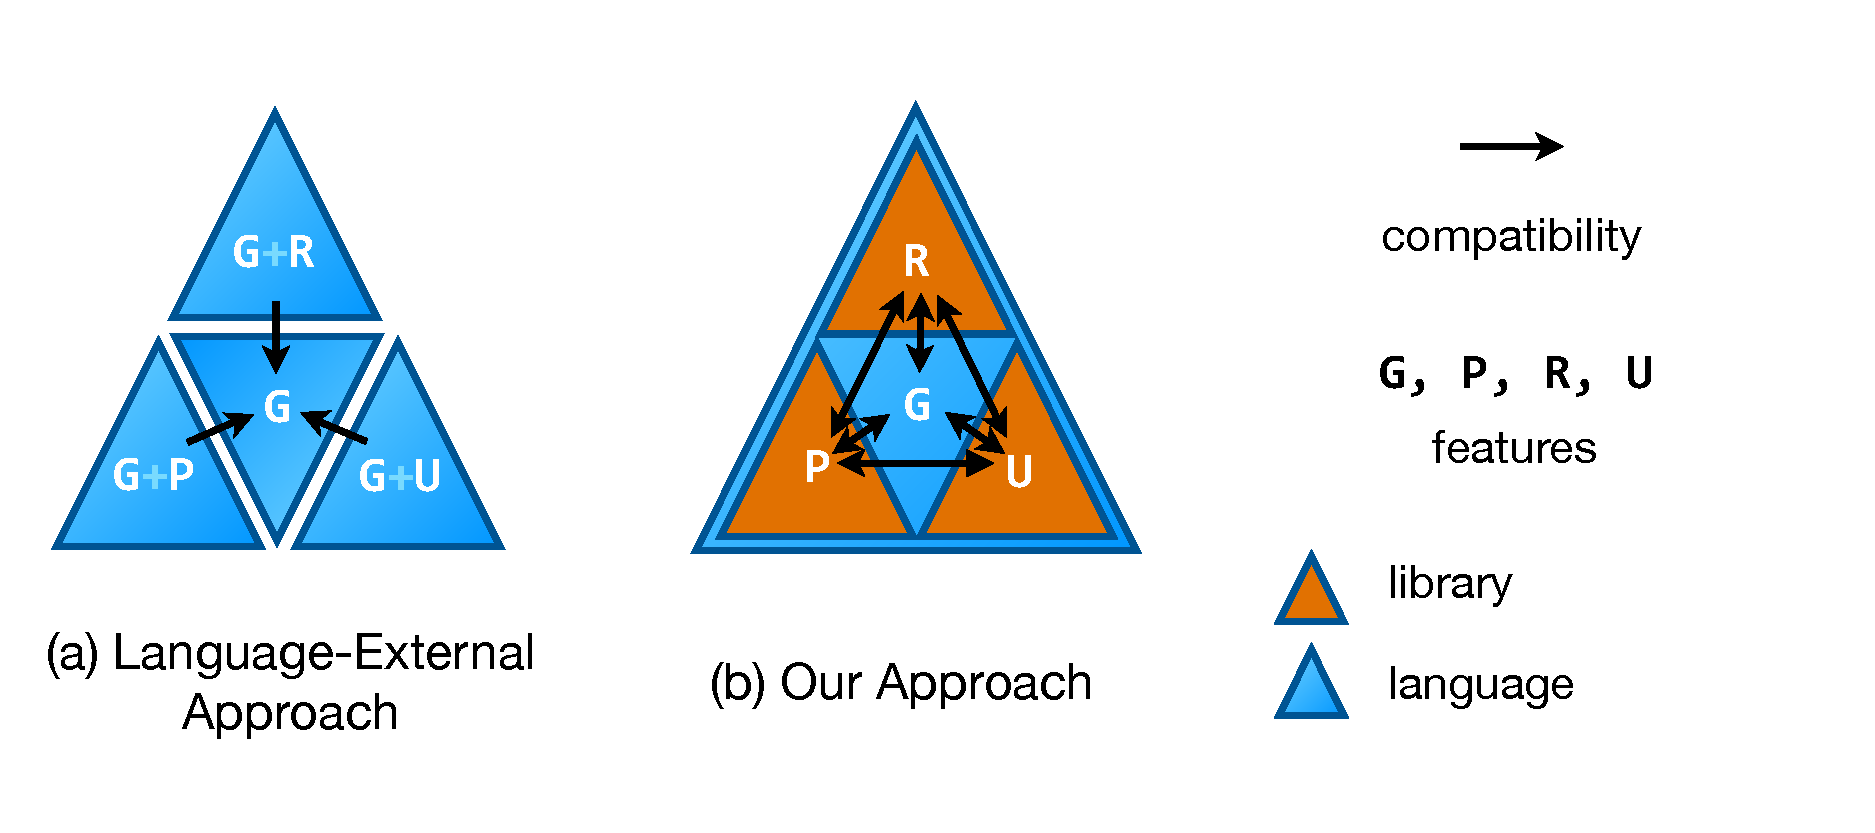
\includegraphics[scale=0.5]{approaches.pdf}
%\end{center}
%\vspace{-20px}
%\caption{\small (a) With a language-oriented approach, novel constructs are packaged into separate languages. Users can only safely and naturally call into languages consisting of common constructs (often only the common target language, such as C or Java bytecode). (b) With a language-internal extensibility approach, there is one system providing a common internal language, where additional primitive constructs that strictly strengthen its static guarantees or perform specialized code generation are specified and distributed within libraries. \label{approaches}}
%\end{figure*}

%As a result, domain-specific languages and new general-purpose abstractions alike have experienced relatively slow adoption in practice.
%
%Porting large codebases to new languages is difficult, and the dominant programming languages innovate slowly, so programming language.
%
%More specifically, such languages are neither \emph{internally extensible} because the language itself exposes only natural numbers and functions to its users, nor are they \emph{externally extensible} because no new behaviors can be added to the language's  implementation in a separate module from the one containing the initial implementation.

%This is the essence of a monolithic language implementation: it is impossible for anyone to modularly extend languages defined in this way. 

An extensible programming language could address these problems by providing a language-integrated mechanism for introducing new type and operator constructors and implementing their associated static and dynamic semantics directly. 
%Library developers need only consider which abstractions are most appropriate for their domain, without also considering whether these constructs can be exposed using abstractions appropriate to the domains of client code. Clients can simply import any necessary constructs when using a library that relies on them, preserving safety and ease-of-use without the use of  wrappers and glue code. We show this competing approach in Figure \ref{approaches}(b).
%Researchers and domain experts thus gain the ability to distribute new ideas for evaluation to a broader development community without requiring the approval of maintainers of mainstream languages, large-scale porting of code or explicit interoperability layers. 
But, as mentioned in Section \ref{language-integrated-approaches}, some significant challenges must be addressed before such a mechanism can be relied upon. The desire for expressiveness must be balanced against  concerns about maintaining various safety properties in the presence of arbitrary combinations of user-defined  extensions to the language's core semantics. The mechanism must ensure that desirable \emph{metatheoretic properties} (e.g. type safety, decidability) of the language are maintained by extensions. Because multiple independently developed extensions might be used within one program, the mechanism must further guarantee their \emph{non-interference}. These are the issues we seek to address in this work.
%\subsection{Theory}\label{atlam}
%%\begin{figure}
%%\begin{mathpar}
%%\inferrule{a}{b}
%%\end{mathpar}
%%\end{figure}
%In this section, we will describe a minimal calculus that captures our language-internal extensibility mechanism,  called \emph{active typechecking and translation (AT\&T)}. AT\&T allows developers to declare new primitive type families, associate operators with them, implement their static semantics in a functional style, and realize their dynamic semantics by simultaneously implementing a translation into a typed internal language. Note that this latter mechanism is closely related to how Standard ML was (re-)specified\todo{cite/read a bit about this/ask Bob/flesh this out}, but that we are fundamentally interested in extending language \emph{implementations}, not their  declarative specifications; proving the adequacy of such implementations against mechanized specifications, or extracting them directly from such specifications, will be investigated in future work.
%
%The AT\&T mechanism utilizes type-level computation of higher kind and integrates typed compilation techniques into the language to allow us to give strong metatheoretic guarantees,  and uses a mechanism notionally related to abstract types (such as those found in the ML module system) to guarantee that extensions cannot interfere with one another,  while remaining straightforward and expressive. In this section, we will develop a core calculus, called \atlam, which uses a minimal, uniform grammar for primitive operators. Then in Section \ref{ace}, we will show how to realize this minimal mechanism within a widely-used language with a more expressive grammar.
%
%AT\&T is general with respect to many choices about the type-level language, the typed internal language and syntax. Choices along these dimensions can affect both expressiveness and ease-of-use. We will begin in Sec. 2 by introducing a minimal system called $@\lambda$ (the ``actively-typed lambda calculus'') that distills the essence of the mechanism in a simply-typed, simply-kinded setting. This will allow us to fully and concisely formalize the language and compiler and give several key safety theorems. We will then continue in Sec. 3 by discussing variants of this mechanism based on other basic paradigms, considering dependently-typed functional languages and object-oriented languages, discussing trade-offs between expressivity and safety when doing so. We have developed a simple prototype called Ace and have used it to develop a number of full-scale language extensions as libraries. We will briefly discuss this language and these extensions in Sec. 4.

%We note at the outset that AT\&T focuses on extending the static semantics of languages with fixed, though flexible, syntax. Language-internal syntax extension mechanisms have been developed in the past (e.g. SugarJ \cite{sugarj}) but they have also suffered from safety problems because grammar composition is not always safe when done in an  unconstrained manner. Tyconstrained approaches that provide stronger safety guarantees have recently been outlined (e.g. Wyvern \cite{globaldsl13}) but we will leave integration of syntax extensions with semantic extensions as future work.

\subsubsection{From Extensible Compilers to Extensible Languages}\label{evolution}
The monolithic character of most programming languages is reflected in, and perhaps influenced by, the most common mechanisms used for implementing programming languages.
Let us consider an implementation of the STLC. 
A compiler written using a functional language will invariably represent the primitive type  and operator constructors using {closed} recursive sums. 
A simple implementation in Standard ML could be based around these datatypes, for example:
\begin{lstlisting}
  datatype Type = Arrow of Type * Type
  datatype Exp = Var of var | Lam of var * Type * Exp | Ap of Exp * Exp 
\end{lstlisting}

The compiler front-end, which consists of a typechecker and translator to a suitable intermediate language (for subsequent compilation by some suitable back-end), will proceed by exhaustive case analysis over the constructors of \lstinline{Exp}.

In a class-based object-oriented implementation of Godel's T, we might instead encode type and operator constructors as subclasses of abstract classes \lstinline{Type} and \lstinline{Exp}. Typechecking and translation, however, will proceed by the ubiquitous \emph{visitor pattern}, dispatching against a fixed collection of {known} subclasses of \lstinline{Exp}.

In either case, we encounter the same basic issue: there is no way to modularly add new primitive type and operator constructors to \li{Type} and \li{Exp}, respectively, and provide implementations of their associated typechecking and translation logic. Everything is defined in precisely one place.
%This issue is related to the widely-discussed \emph{expression problem} (in a restricted sense -- we do not consider adding new functions beyond typechecking and translation here, only adding logic to these) \cite{wadler-expression}.

A number of language mechanisms have been proposed that allow new cases to be added to datatypes and the functions that operate over them in a modular manner. 
In functional languages, we might use \emph{open datatypes} \cite{opendatatypes}\todo{cite}. For example, if we wish to extend our implementation of the STLC with product types and we have written our compiler in a language supporting open datatypes, it might be possible to add new constructors: 
\begin{lstlisting}
  newcon Prod of Type * Type extends Type
  newcon Pair of Exp * Exp extends Exp
  newcon PrL of Exp extends Exp
  newcon PrR of Exp extends Exp
\end{lstlisting}

The logic for functionality like typechecking and translation can then be implemented for only these new cases. For example, the \lstinline{typeof} function that synthesizes a type for an expression given a context could be extended to support the new case \li{PrL} like so:
\begin{lstlisting}
  typeof (ctx, PrL(e)) = case typeof (ctx, e) of 
      Prod(t1, _) => t1 
    | _ => raise TypeError("<appropriate error message>")
\end{lstlisting}

If we allowed users to define new modules containing definitions like these and link them into our compiler, we will have succeeded in creating an externally-extensible compiler, albeit one where safety and non-interference is not guaranteed (we will return to this point shortly). We have not, however, created an extensible programming language because other compilers for the same language will not necessarily support the same extensions. 
If our newly-introduced constructs are exposed at a library's  interface boundary, clients of that library who are using different compilers face the same problems with client compatibility that those using different languages face (as described in Sec. \ref{external-approaches}). That is, {extending a language by extending a single compiler for it is morally equivalent to creating a new language}. 

We argue that a more appropriate and useful place for extensions like this is directly within libraries, alongside abstractions that can be implemented in terms of existing primitive abstractions. To enable this, the language must allow for the introduction of new type constructors, like \lstinline{Prod}, operator constructors, like \lstinline{Pair}, \lstinline{PrL} and \lstinline{PrR}, and their associated type synthesis and translation logic. Because this mechanism is integrated into the language specification, all compilers must support it.

The design described above suggests we may now need to add another layer to our language, above the type-level language (conventionally, $\tau$) and expression language (conventionally, $e$), where extensions are implemented. In fact, we will show that \textbf{a natural place for type system extensions is within the type-level language}. The intuition  is that extensions to a statically typed language's semantics will need to manipulate types as values at compile-time. Many languages already allow users to write type-level functions for various reasons, effectively supporting this notion of types as values at compile-time. The type-level language is often constrained by its own type system, where the types of type-level terms are called \emph{kinds} for clarity,  that prevents type-level functions from causing problems during compilation. The kind system is often more constraining than the type system is (e.g. it might permit only terminating functions, to ensure that typechecking is decidable). This is precisely the structure that a distinct extension layer would have, and so we will show that is quite natural to unify the two.


\subsubsection{@$\lambda$: Conservatively Extending a Type System From Within}
\begin{figure}[t]
\small
$$\begin{array}{rccl}	
\textbf{programs} & \rho & ::= & \pfam{\familyDf}{\progsort} \pipe \pdef{t}{\kappa}{\tau}{\progsort} \pipe e\\
\text{operators}		&	\theta	&	::= &	\tops{op}{\kappaidx}{i}{a}{\taut{def}} \pipe 
												\topp{\theta}{\theta}\\
\\
\textbf{external terms} 				&	e	&	::=	&	\evar{x} \pipe 
														\elam{\evar{x}}{\tau}{e} \pipe 
														\eop{Tycon}{op}{
															\tauidx
														}{
  												    		\splat{e}{1}{n}
														} \\
									& 		&		& 	\\
							
\hspace{-5pt}\textbf{type-level terms} 	& \tau 	& ::= 	& 	\tvar{t} \pipe 
														\tlam{t}{\kappa}{\tau} \pipe 
														\tapp{\tau_1}{\tau_2} \pipe
														\tnil{\kappa} \pipe \tcons{\tau_1}{\tau_2} \pipe 
									                     \tfold{\tau_1}{\tau_2}{h}{t}{r}{\tau_3}
														\\
												
\text{type-level data}	 			& 		& \pipe	& 	 \iintlit \pipe \iop{\tau_1}{\tau_2} \pipe \tstr{str} \pipe \tunit \pipe 
														\tpair{\tau_{1}}{\tau_{2}} \pipe 
														\tfst{\tau} \pipe 
														\tsnd{\tau} 
														\\	

\text{types} 						& 		& \pipe	& 	\ttypestd \pipe \tfamcase{\tau}{Tycon}{x}{\tau_1}{\tau_2}\\
						%				& & \pipe & \tfamcase{\tau}{Fam}{x}{\tau_1}{\tau_2}\\
\text{structural equality}  & & \pipe & 					\tifeq{\tau_{1}}{\tau_{2}}{\kappa}{\tau_{3}}{\tau_{4}} 
														\\																																					
\text{elaborations} 				& 		 & 	\pipe	&	\tden{\tauiterm}{\tautype} \pipe \terr \pipe \tdencase{\tau}{x}{t}{\tau_1}{\tau_2}\\
 %& & \pipe & 
%														\tdencase{\tau}{y}{x}{\tau_1}{\tau_2}
%														 \\

\text{reified IL}		&		&	\pipe	&	\titerm{\iota} \pipe \titype{\sigma} \\

												\\
\textbf{kinds} 					& \kappa	&	::=	&	\karrow{\kappa_1}{\kappa_2} \pipe \klist{\kappa} \pipe \dint \pipe
											    \kstr \pipe
												\kunit \pipe 
												\kpair{\kappa_{1}}{\kappa_{2}} \pipe 
												\kTypeBlur \pipe \kDen \pipe 
												\kITerm \pipe \kIType
												\\
\\												
%\textbf{ops signature}			& \Theta	&	::=	&	\kOpEmpty \pipe \kOp{\Theta}{op}{\kappai}\\
%											 							&		&		&	\\
\textbf{internal terms} 				& 	\iota	&	::=	&	\evar{x} \pipe 
												\ilam{\evar{x}}{\sigma}{\iota} \pipe 
												\iapp{\iota_{1}}{\iota_{2}} \pipe
												\ifix{\evar{f}}{\sigma}{\iota} \pipe
												\ipair{\iota_{1}}{\iota_{2}} \pipe 
												\ifst{\iota} \pipe
												\isnd{\iota}
												\\
							& 		& 	\pipe	& 
												\iintlit \pipe \iop{\iota_{1}}{\iota_{2}} \pipe \iIfEq{\iota_{1}}{\iota_{2}}{\dint}{\iota_{3}}{\iota_{4}}  
												\\
 &  & \pipe & \tvalof{\tau_1}{\tau_2} \pipe \iup{\tau} \\
%\text{deabstracted}& \iota & ::= & \mathcal{G}[\iota, \sigma]\\
\textbf{internal types}			&	\sigma	&	::=	&    \darrow{\sigma_1}{\sigma_2} \pipe
												\dint \pipe
												\dpair{\sigma_1}{\sigma_2} \pipe
												\trepof{\tau} \pipe \dup{\tau}\\
\end{array}$$
\vspace{-10pt}
\caption{\small Abstract syntax of \atlam. Here, $x$ ranges over external and internal language variables, $\tvar{t}$ ranges over type-level variables, $\fvar{Tycon}$ ranges over type constructor names and $\opvar{op}$ ranges over operator constructor names. The form $\tstr{str}$ represents string literals, $\iintlit$ represents integer literals and $\oplus$ represents standard total binary operations over integers.%The productions related to the internal language are written using generators $\mathcal{G}$ and $\mathcal{S}$ to avoid duplicating the syntax of common terms.
\label{grammar}}
\end{figure}
\begin{figure}[t]
\begin{lstlisting}
tycon Nat of 1 with  
    schema $\lambda$idx:1.$\blacktriangledown$($\mathbb{Z}$) 
    opcon Z of 1 ($\lambda$idx:1.$\lambda$args:list[Elab].is_empty args $\llbracket$$\triangledown$(0) as Nat[()]$\rrbracket$)
    opcon S of 1 ($\lambda$idx:1.$\lambda$args:list[Elab].pop_final args $\lambda$x:ITm.$\lambda$ty:$\star$. 
      checktype ty Nat[()] $\llbracket$$\triangledown$($\vartriangle$(x)+1) as Nat[()]$\rrbracket$)
    opcon Rec of 1 ($\lambda$idx:1.$\lambda$args:list[Elab].
      pop args $\lambda$x1:ITm.$\lambda$ty1:$\star$.$\lambda$args':list[Elab].
      pop args' $\lambda$x2:ITm.$\lambda$ty2:$\star$.$\lambda$args'':list[Elab].
      pop_final args'' $\lambda$x3:ITm.$\lambda$ty3:$\star$.
      check_type t1 Nat[()] (
      check_type t3 Arrow[(Nat[()], Arrow[(t2, t2)])] 
      	$\llbracket$$\triangledown$((fix f:$\mathbb{Z} \rightarrow$ rep(t2) is $\lambda$x:$\mathbb{Z}$.
	        if x = 0 then $\vartriangle$(x2) else $\vartriangle$(x3) (x - 1) (f (x - 1))) $\vartriangle$(x1)) as t2$\rrbracket$))
end
\end{lstlisting}
\caption{An implementation of primitive natural numbers as internal integers in @$\lambda$.}
\label{nat-atlam}
\end{figure}
We will begin by developing an ``actively-typed'' version of the simply-typed lambda calculus with type-level computation called @$\lambda$. In the semantics for this calculus, we will integrate typed compilation techniques and a form of type abstraction to allow us to prove key type safety and non-interference theorems. The abstract syntax of @$\lambda$ is in Fig. \ref{grammar}. 

The semantics of the language are in the style of the Harper-Stone elaboration semantics for Standard ML: all terms in an external language, $e$, are simultaneously assigned a type and an elaboration to a term, $\iota$, in a fixed typed internal language \cite{HarperStone, Stone}. The mechanism checks that any generated elaborations are \emph{type preserving} -- that all external terms of a particular type, $\tau$, elaborate to internal terms with a consistent internal type, $\sigma$ -- following the approach taken in the TIL compiler for Standard ML by Morrisett et al. \cite{TIL}. This allows the semantics to be reasoned about compositionally and, when combined with type safety of the internal language, gives us type safety of the extensible external language. 
This design ensures that global properties that the internal language maintains are guaranteed to hold no matter which extensions are introduced. In other words, extension providers cannot implement type systems weaker than the type system of the internal language. Providers are, however, able to implement type systems that maintain invariants stronger than those the internal type system can maintain. The internal language of @$\lambda$ is PCF with simple products and one base type, integers. Because of the availability of the fixpoint operator, the internal language is universal (i.e. Turing-complete).

It is reasonable, if we wish to actually implement this language, to permit only the addition of deterministic, decidable rules to the semantics. Extension logic is thus implemented in a functional style  (essentially, lifting fragments of the typechecker into the type-level language), rather than extracted from inductive specifications, like those in the Sec. \ref{foundations}\footnote{Though we will not explore this further in this thesis, a system for extracting such a function from a declarative specification could potentially be implemented using the techniques in Sec. \ref{aparsing} -- a \emph{kind-specific language}!}. This has the added benefit of giving providers finer-grained control over error reporting. When extracting an implementation from a typical inductive specification, which only specifies ``success conditions'', it is difficult to provide different error messages at different failure points within a single rule.
%In this section, we will sketch a calculus where new type families and operator families can be introduced by users. The type synthesis and translation logic that implements the desired static and dynamic semantics, respectively, for these is implemented in the type-level language. 

To give a first example, the code in Fig. \ref{nat-atlam} (written using concrete syntax) shows how to introduce a new type constructor, $\fvar{Nat}$, indexed trivially (i.e. by a type-level value of kind 1, also known as unit). Types themselves are type-level values of kind $\kTypeBlur$ and are introduced by naming a type constructor and providing an index of the appropriate kind: $\ttype{Nat}{\tunit}$. To ensure that type equality is decidable, type constructors can only be indexed by values of a kind for which equality is ``trivially'' decidable (i.e. where semantic equality coincides with syntactic equality). This means that types themselves, as well as type-level data structures containing values of equality kind, can be used, while type-level functions cannot.

To ensure that compilation is type-preserving, as described above, each type must have an internal type, called its \emph{representation}, associated with it. The representation of a type might depend on its index, so each type constructor must declare a type-level function that returns an internal type given an index, called its \emph{representation schema}. An internal type, $\sigma$, is reflected into a type-level terms of kind $\kIType$ via the introductory form $\blacktriangledown(\sigma)$. Because $\fvar{Nat}$ is indexed trivially, it simply returns the reflected form of the internal type $\mathbb{Z}$. %The sort $\sigma$ also contains forms $\trepof{\tau}$ and $\dup{\tau}$. The former allows one to refer, abstractly, to the representation of the type $\tau$, while the latter enables the interpolatation of a type-level value of kind $\kIType$.

%Two additional forms, $\tvalof{\tauiterm}{\tautype}$ and $\iup{\tau}$, will be discussed below. These are erased by the end of the elaboration process.

In the external language, $e$, all operators (other than $\lambda$, for reasons we will discuss) are invoked uniformly. The natural number two, for example, is written: $$\eop{Nat}{s}{()}{\eop{Nat}{s}{()}{\eop{Nat}{z}{()}{ }}}$$

Operator constructors, like type constructors, are indexed by type-level values. In our example, all the operators are indexed trivially, but we will see examples later where non-trivial operator indices are useful. We will discuss why operator constructors are associated directly with type constructors, rather than existing as standalone entities, when we discuss the scoping mechanism for the representation schema, which is essential for guaranteeing non-interference. This coupling also forms the foundation for a higher-level elaboration mechanism that allows us to use more conventional and concise (though still fixed) syntactic idioms, which we intend to explore in this thesis, but have not yet formalized. For now, we simply note that intuitively, most operators are either introduction or elimination forms for a particular type, so we are simply encoding a common idiom. 

The declarations of the three operator constructors related to natural numbers are given on lines 3-13 of Fig. \ref{nat-atlam}. Operator constructors are declared by specifying the kind of type-level value they are indexed by and giving an \emph{operator definition}, a type-level function of kind $\kappa \rightarrow \klist{\kDen} \rightarrow \kDen$. The kind $\kDen$ classifies \emph{elaborations}. There are two introductory forms for this kind: \emph{valid elaborations}, $\tden{\tauiterm}{\tautype}$, consist of a reflected internal language term paired with a type assignment, while \emph{error elaborations}, $\terr$, represent a type error (in a full implementation, the error elaboration would contain an error message, as discussed above, but for simplicity in our core calculus, we simply treat all type errors equivalently). Internal terms, $\iota$, like internal types, are reflected as type-level terms of kind $\kITerm$ via the introductory form $\titerm{\iota}$. The form $\iup{\tau}$ interpolates a type-level value of kind $\kITerm$ into an internal term.  Note that there are no elimination forms for the kinds $\kIType$ and $\kITerm$. Composition occurs entirely via interpolation -- syntax trees are never examined directly by extensions in @$\lambda$. 

Operator definitions are called by the compiler to generate an elaboration for operator invocations. In our example, the definition of $\fvar{Nat}.\opvar{z}$ simply checks that there were no arguments (using a simple helper function for working with lists of elaborations, \li{is_empty}, not shown) and if so, provides an elaboration where the internal language integer \li{0} is associated with type $\ttype{Nat}{\tunit}$. If the list is not empty, \li{is_empty} simply returns $\terr$. The other two operator constructors are more verbose, but follow a similar pattern -- elaborations are popped off and broken down into their constituent internal terms and types by helper functions, then a functional program that implements the intended semantics is written to produce an elaboration as a whole. Note that the \li{Rec} operator does not itself bind new variables; it must use the built-in \li{Arrow} type constructor. There is no support in @$\lambda$ for introducing new forms of binding; $\lambda$ is the only available binding operator. Note that application is invoked like other operators: $\eop{Arrow}{ap}{\tunit}{e_1; e_2}$.

This definition of natural numbers can be shown to be an adequate encoding of the semantics given in Sec. \ref{foundations}. It can also be shown to maintain the invariant that natural numbers elaborate into \emph{non-negative} internal integers. Note that because we are beginning with a simply-typed, simply-kinded formulation, these kinds of statements must be proven metatheoretically (as with other sorts of complex invariants in simply-typed languages). With a naive formulation of this mechanism, these theorems would be quite a bit more precarious, however. If another provider, perhaps a malicious one, declares a new operator constructor that introduces natural numbers, these theorems may not be \emph{conserved}. For example, the following operator declaration is quite problematic:

\begin{lstlisting}
opcon badnat of 1 ($\lambda$idx:1.$\lambda$args:list[Elab].$\llbracket\triangledown$(-1) as Nat[()]$\rrbracket$)
\end{lstlisting}

With this declaration, there is now a new and unexpected introductory form for the natural number type, and even worse, it violates our previous implementation invariants. A naive check for type preservation would not catch this problem: \li{-1} does have type $\mathbb{Z}$, it is simply not an integer that could have been emitted by the original definition of \li{Nat}.

To prevent this problem, we \emph{hold the representation of a type abstract} outside of the operators explicitly associated with it. If \li{badnat} cannot know that the representation of \li{Nat[()]} is $\mathbb{Z}$, then the above operator implementation cannot be correct. Because we cannot prove relational correctness properties from within a simply-typed/kinded calculus, our semantics enforces this by using a form of value abstraction, similar to that described by Zdancewic et. al \cite{zdancewic}. In brief: the representation of a type, written $\trepof{\tautype}$, does not reduce further to the actual representation type (e.g. to $\mathbb{Z}$) when not in an operator definition associated with $\tautype$. The only internal form that can be checked against  $\trepof{\tautype}$ is the special form $\tvalof{\tauiterm}{\tautype}$, an abstracted internal term corresponding to the internal term reflected by $\tauiterm$. Rather than exposing it explicitly, it is wrapped so that it can't be checked against any type other than $\trepof{\tautype}$. A full description of this mechanism (and the others, described above) requires us to introduce the semantics in detail. A draft of the semantics of @$\lambda$ is available as a paper draft\footnote{\url{https://github.com/cyrus-/papers/tree/master/esop14}}.


The use cases permitted by this mechanism are not simply subsumed by a module system with support for abstract types and functors. Indeed, such a module system is an orthogonal concern in that it must sit atop a core type system. More particularly, the distinction is the fundamental one between functions and operators. Functions cannot examine type indices at compile-time to determine a return type and implementation (or generate static error messages), as operators are able to do. It is encouraging that there are clear parallels between module systems with abstract types and type constructors with abstract schemas, and any full-scale language design based on this mechanism should certainly provide both mechanisms (with the former used in most cases). We plan to investigate this relationship more thoroughly, showing examples where abstract types are more clearly unsuitable, in the remainder of this work. 


\subsubsection{Remaining Tasks and Timeline}
We are actively working on this mechanism and plan to submit a paper to ICFP 2014 on Mar. 1 based on a submission to ESOP 2014 that was not accepted. The following key tasks, other than clarifying the writing, remain to be completed:

\begin{enumerate}
\item Reviewers of the previous submission to ESOP found a problem with our treatment of internal type variables that needs to be corrected by threading a context through the type-level evaluation semantics.
\item We must more rigorously state and prove the key lemmas and theorems related to type preservation, type safety, decidability and conservativity. 
\item We must develop examples that are more interesting than natural numbers. In particular, some interesting form of labeled product type that SML doesn't have (e.g. a record with prototypic dispatch) as well as sum types would be interesting.
\item We must consider whether properties related to termination can be conserved by this mechanism, because a fixpoint can be used to introduce a non-terminating expression of any type. This may be possible by being careful about how deabstraction interacts with fixpoints.
\item We must more clearly connect this work to the Harper-Stone semantics and other related work, and clarify  the relationship to abstract types.
\item We must show how to add additional syntactic forms to the external language that defer to the generic operator invocation form in a type-directed manner. This connects the theory to the work on Ace, described below. 
\end{enumerate}

\subsection{Ace}\label{ace}
\lstset{
  language=Python,
  showstringspaces=false,
  formfeed=\newpage,
  tabsize=4,
  commentstyle=\itshape,
  basicstyle=\ttfamily\scriptsize,
  morekeywords={lambda, self, assert, as},
  numbers=left,
  numberstyle=\scriptsize\color{light-gray}\textsf,
  xleftmargin=2em,
  stringstyle=\color{mauve}
}
\lstdefinestyle{Bash}{
    language={}, 
    numbers=left,
    numberstyle=\scriptsize\color{light-gray}\textsf,
    moredelim=**[is][\color{blue}\bf\ttfamily]{`}{`}
}
\lstdefinestyle{OpenCL}{
	language=C++,
	morekeywords={kernel, __kernel, global, __global, size_t, get_global_id, sin, printf, int2}
}

%\usepackage{float}
%\floatstyle{ruled}
%\newfloat{codelisting}{tp}{lop}
%\floatname{codelisting}{Listing}
%\setlength{\floatsep}{10pt}
%\setlength{\textfloatsep}{10pt}



The key choices that a language must make when supporting the mechanism described in the previous section are:
\begin{enumerate}
\item What is the semantics of the type-level language?
\item What is the syntax of the external language, and how should the syntactic forms dispatch to  operator definitions?
\item What is the semantics of the internal language?
\end{enumerate}

In @$\lambda$, the type-level language was a form of the simply-typed lambda calculus with a few common data types, and the internal language was a variant of PCF. The external language currently only includes direct dispatch by naming an operator explicitly. This is useful for the purposes of clarifying the foundations of our work.

In this section, we wish to explore a different point in this design space, with an eye toward practicality and expressiveness. In particular, we want to show how to implement {the extension mechanism itself} as a library within an existing, widely used language, solving a \emph{bootstrapping problem} that has prevented  other work on extensibility from being effective as a means to bring more research into practice. This language, called Ace, makes the following choices:

\begin{enumerate}
\item Python is used as the type-level language (and more generally, as a compile-time metalanguage).
\item Python's syntax is used for the external language. We will describe the dispatch protocol below.
\item The internal language can be user-defined, rather than being pre-defined as in @$\lambda$.
\end{enumerate}

The choice of Python as the host language presents several challenges because we are attempting to embed an extensible static type system within a uni-typed (a.k.a. dynamically typed) language, without modifying its syntax in any way. We show that by leveraging Python's support for function quotations and by using its class-based object system to encode type constructors, we are able to accomplish this goal. Then, with a flexible statically-typed language under the control of libraries, we implement a variety of statically-typed abstractions, including common functional abstractions (e.g. inductive datatypes with pattern matching), low-level parallel abstractions (all of the OpenCL programming language), object systems and domain-specific abstractions (e.g. regular expression types, as described in the introduction). Ace can be used both as a standalone language and as a staged compilation environment from within Python.

\subsubsection{Language Design and Usage}\label{usage}
Listing \ref{map} shows an example of an Ace file. As promised, the top level of an Ace file is written directly in Python, requiring no modifications to the language (versions 2.6+ or 3.3+) nor features specific to CPython (so Ace supports alternative implementations like Jython, IronPython and PyPy). This choice pays  dividends on line 1: Ace's package system is Python's package system, so Python's build tools (e.g. \verb|pip|) and package repostories (e.g. \verb|PyPI|) are directly available for distributing Ace libraries. 

The top-level statements in an Ace file, like the \verb|print| statement on line 10, are executed at compile-time. That is, Python serves as the \emph{compile-time metalanguage} of Ace. %For readers familiar with C/C++, Python can be thought of as serving a role similar to (but more general than) its preprocessor and template system (as we will see).
Functions containing run-time behavior, like \verb|map|, are annotated as Ace functions and are then governed by a semantics that differs substantially from Python's (in ways that we will describe below). But Ace functions share Python's syntax. As a consequence, users of Ace benefit from an ecosystem of well-developed tools that work with Python syntax, including parsers, code highlighters, editor modes, style checkers and documentation generators. 

\subsubsection{OpenCL as an Active Library}
The code in this section uses \verb|clx|, an example of an library that implements the semantics of the OpenCL programming language, and extends it with some additional useful types, using Ace. Ace itself has no built-in support for OpenCL.

To briefly review, OpenCL provides a data-parallel SPMD programming model where developers define functions, called {\em kernels}, for execution across thousands of threads on \emph{compute devices} like GPUs or multi-core CPUs \cite{opencl11}. Each thread has access to a unique index, called its \emph{global ID}. Kernel code is written in the OpenCL kernel language, a somewhat simplified variant of C99 extended with some new primitive types and operators, which we will describe as needed in our examples below.

\subsubsection{Generic Functions}\label{genfn}
\begin{codelisting}
\lstinputlisting{../ace-pldi14/listing3.py}
\caption{[\texttt{listing\ref{map}.py}] A generic imperative data-parallel higher-order map function targeting OpenCL.}
\label{map}
\end{codelisting}
%\begin{codelisting}
%\lstinputlisting[commentstyle=\color{mauve}]{../ace-pldi14/listing7.py}
%\caption{[\texttt{listing\ref{metaprogramming}.py}] Metaprogramming with Ace, showing how to construct generic functions from abstract syntax trees.}
%\label{metaprogramming}
%\end{codelisting}
%\begin{codelisting}
%\begin{lstlisting}[style=Bash]
%$ `acec listing3.py`
%Hello, compile-time world!
%[ace] TypeError in listing1.py (line 6, col 28): 
%      'GenericFnType(negate)' does not support [].
%[acec] listing3.cl successfully generated.
%\end{lstlisting}
%\caption{Compiling \texttt{listing\ref{compscript}.py} using the \texttt{acec} compiler.}
%\label{mapc}
%\end{codelisting}
%\begin{codelisting}
%\lstinputlisting[style=OpenCL]{listing5.cl}
%\caption{[\texttt{listing\ref{compscript}.cl}] The OpenCL file generated by Listing \ref{mapc}.}
%\label{mapout}
%\end{codelisting}

Lines 3-4 introduce \verb|map|, an Ace function of three arguments that is governed by the \emph{active base} referred to by \verb|clx.base| and targets the \emph{active target} referred to by \verb|clx.opencl|. The active target determines which language the function will compile to (here, the OpenCL kernel language) and mediates code generation. The active target plays an analagous role to the internal language of @$\lambda$.

The body of this function, on lines 5-8, does not have Python's semantics. Instead, it will be governed by the active base together with any \emph{active types} used within it. No  types have yet been assigned, however. Because our type system is extensible, the code inside could be meaningful for many different assignments of types to the arguments (a form of \emph{ad hoc polymorphism}). We call functions awaiting types, like \verb|map|,  \emph{generic functions}. Once types have been assigned, they are called \emph{concrete functions}.

Generic functions are represented at compile-time as instances of \verb|ace.GenericFn| and consist of an abstract syntax tree, an {active base}, an {active target} and a read-only copy of the Python environment that they were defined within. The purpose of the \emph{decorator} on line 3 is to replace the Python function on lines 4-8 with an Ace generic function having the same syntax tree and environment and the provided active base and active target. 
A decorator in Python is simply syntactic sugar that applies another function directly to the function  being decorated \cite{python}. In other words, line 3 could be replaced by the following  statement on line 9: \verb|map = ace.fn(clx.base, clx.opencl)(map)|.
Ace extracts the abstract syntax tree for \verb|map| using the Python standard  library packages  \verb|inspect| (to retrieve its source code) and \verb|ast| (to parse it into a syntax tree). The ability to extract a function's syntax tree and inspect its closure directly are the two key ingredients for implementing a mechanism like this as a library within another language.

\subsubsection{Concrete Functions and Explicit Compilation}
\begin{codelisting}
\begin{lstlisting}
import listing1, ace, examples.clx as clx

@ace.fn(clx.base, clx.opencl)
def negate(x):
  return -x

T1 = clx.Ptr(clx.global_, clx.float)
T2 = clx.Ptr(clx.global_, clx.Cplx(clx.int))
TF = negate.ace_type

map_neg_f32 = listing1.map[[T1, T1, TF]]
map_neg_ci32 = listing1.map[[T2, T2, TF]]
\end{lstlisting}
%\lstinputlisting{../ace-pldi14/listing4.py}
\caption{[\texttt{listing2.py}] The generic \texttt{map} function compiled to map the \texttt{negate} function over two  types of input.}
\label{compscript}
\end{codelisting}

To compile a generic function to a particular \emph{concrete function}, a type must be provided for each argument, and typechecking and elaboration must then succeed. Listing \ref{compscript} shows how to explicitly provide type assignments to \verb|map| using the subscript operator (implemented using Python's operator overloading mechanism). We do so two times in Listing \ref{compscript}, on lines 11 and 12. Here, \verb|T1|, \verb|T2|, \verb|TF|, \verb|clx.float|, \verb|clx.int| and \verb|negate.ace_type| are types and \verb|clx.Ptr| and \verb|clx.Cplx| are type constructors. We will discuss these in the next section.
 
Concrete functions like \verb|map_neg_f32| and \verb|map_neg_ci32| are instances of \verb|ace.ConcreteFn|. They consist of a \emph{typed} abstract syntax tree, an elaboration into the target language and a reference to the originating generic function. %The typing and translation process is mediated by the logic in the active base, types and target that have been provided, as we will describe in more detail below. 

To produce an output file from an Ace ``compilation script'' like \verb|listing|\texttt{\ref{compscript}}\verb|.py|, the command \verb|acec| can be invoked from the shell, as shown in Listing \ref{mapc}. The result of compilation is the OpenCL file shown in Listing \ref{mapout}. The \verb|acec| compiler (a simple Python script) operates in two stages:
\begin{enumerate}
\item Executes the provided Python file (\verb|listing3.py|).
\item Extracts the elaborations from concrete functions and other top-level constructs that define elaborations (e.g. types requiring declarations) in the final Python environment.  This may produce one or more files, depending on which active targets were used (here, just \verb|listing3.cl|, but a web framework built upon Ace might produce separate HTML, CSS and JavaScript files).
\end{enumerate}

%In this case, stage 1 results in the output on lines \ref{mapc}.2-\ref{mapc}.4. The type error printed on lines \ref{mapc}.3-\ref{mapc}.4 will be explained in the next section. The compiler then enters stage 2 and concludes with the message on line \ref{mapc}.5 to indicate that one file was generated. This file is shown in Listing \ref{mapout} and can be used by any programs that consume OpenCL code (e.g. a C program that invokes the generated kernels via the OpenCL host API). 
We will show in the thesis, but omit in this proposal, that for targets with Python bindings, such as OpenCL, CUDA, C, Java or Python itself, generic functions can be executed directly, without any of the explicit compilation steps in Listings \ref{compscript} and \ref{mapc}. This represents a form of staged compilation.  In this setting, the dynamic type of a Python value determines, at the point of invocation, a static type assignment for the argument of an Ace generic function. 

\subsubsection{Types}
\begin{codelisting}
\begin{lstlisting}[style=Bash]
> `acec listing2.py`
Hello, compile-time world!
[acec] listing2.cl successfully generated.
\end{lstlisting}
%$ `acec listing3.py`
%Hello, compile-time world!
%[ace] TypeError in listing1.py (line 6, col 28): 
%      'GenericFnType(negate)' does not support [].
%[acec] listing3.cl successfully generated.
\caption{Compiling \texttt{listing\ref{compscript}.py} using the \texttt{acec} compiler.}
\label{mapc}
\end{codelisting}
\begin{codelisting}
\lstinputlisting[style=OpenCL]{../ace-pldi14/listing5.cl}
\caption{[\texttt{listing\ref{compscript}.cl}] The OpenCL file generated by Listing \ref{mapc}.}
\label{mapout}
\end{codelisting}
Lines 7-9 of Listing \ref{compscript} construct the types used to generate concrete functions from the generic function \verb|map| on lines 11 and 12. In Ace, types are themselves values that can be manipulated at compile-time. Python is thus Ace's type-level language. %This stands in contrast to other contemporary languages, where user-defined types (e.g. datatypes, classes, structs) are written declaratively at compile-time but cannot be constructed, inspected or passed around programmatically. 
More specifically, types are instances of a Python class that implements the \verb|ace.ActiveType| interface. Implementing this interface is analagous to defining a new type constructor in @$\lambda$. 

As Python values, types can be assigned to variables when convenient (removing the need for  facilities like \verb|typedef| in C or \verb|type| in Haskell). Types, like all compile-time objects derived from Ace base classes, do not have visible state and operate in a referentially transparent manner (by constructor memoization, which we do not detail here).% These types are all implemented in the \verb|clx| library imported on line 1, none are built into Ace itself.

The type named \verb|T1| on line 7 directly implements the logic of the underlying OpenCL type \verb|global float*|: a pointer to a 32-bit floating point number stored in the compute device's global memory (one of four address spaces defined by OpenCL \cite{opencl11}). It is constructed by applying \verb|clx.Ptr|, which is an Ace type constructor corresponding to pointer types, to a value representing the  address space, \verb|clx.global_|, and the type being pointed to. That type, \verb|clx.float|, is in turn the \verb|clx| type corresponding to \verb|float| in OpenCL (which, unlike in C99, is always 32 bits). 
The \verb|clx| library contains a full implementation of the OpenCL type system (including  complexities, like promotions, inherited from C99).
Ace is \emph{unopinionated} about issues like memory safety and the wisdom of such promotions. We will discuss how to implement, as libraries, abstractions that are higher-level than raw pointers, or simpler numeric types, but Ace does not prevent users from choosing a low level of abstraction or ``interesting'' semantics if the need arises (e.g. for compatibility with existing libraries). We also note that we are being more verbose than necessary for the sake of pedagogy. The \verb|clx| library includes more concise shorthand for OpenCL's types: \verb|T1| is equal to \verb|clx.gp(clx.f32)|. %Similarly, the decorators in Listings \ref{map} and \ref{metaprogramming} could have been written \verb|clx.cl_fn|.\todo{move this back there probably}

The type \verb|T2| on line 8 is a pointer to a \emph{complex integer} in global memory. It does not correspond directly to a type in OpenCL, because OpenCL does not include primitive support for complex numbers. Instead, the type constructor \verb|clx.Cplx| defines the necessary logic for typechecking operations on complex numbers and elaborating them to OpenCL. This constructor is parameterized by the numeric type that should be used for the real and imaginary parts, here \verb|clx.int|, which corresponds to 32-bit OpenCL integers. Arithmetic operations with other complex numbers, as well as with plain numeric types (treated as if their imaginary part was zero), are supported. When targeting OpenCL, Ace expressions assigned type \verb|clx.Cplx(clx.int)| are compiled to OpenCL expressions of type \verb|int2|, a  \emph{vector type} of two 32-bit integers (a type that itself is not inherited from C99). This can be observed in several places on lines \ref{mapout}.14-\ref{mapout}.21. This choice is merely an implementation detail that can be kept private to \verb|clx|. An Ace value of type \verb|clx.int2| (that is, an actual OpenCL vector) \emph{cannot} be used when a \verb|clx.Cplx(clx.int)| is expected (and attempting to do so will result in a static type error).

The type \verb|TF| on line 9 is extracted from the generic function \verb|negate| constructed in Listing \ref{compscript}. Generic functions, according to Sec. \ref{genfn}, have not yet had a type assigned to them, so it may seem perplexing that we are nevertheless extracting a type from \verb|negate|. Although a conventional arrow type cannot be assigned to \verb|negate|, we can give it a \emph{singleton type}: a type that simply means ``this expression is the \emph{particular} generic function \verb|negate|''. This type could also have been explicitly written as \verb|ace.GenericFnType(listing2.negate)|. During typechecking and translation of \verb|map_neg_f32| and \verb|map_neg_ci32|, the call to \verb|f| on line 6 of Listing \ref{map} uses the type of the argument to generate a concrete function from the generic function that inhabits the singleton type of \verb|f| (\verb|negate| in both cases shown). This is why there are two versions of \verb|negate| in the output in Listing \ref{mapout}. In other words, types \emph{propagate} into generic functions -- we didn't need to compile \verb|negate| explicitly. In effect, this scheme enables higher-order functions even when targeting languages, like OpenCL, that have no support for higher-order functions (OpenCL, unlike C99, does not support function pointers). Interestingly, because they have a singleton type, they are higher-order but not first-class functions. That is, the type system would prevent you from creating a heterogeneous list of generic functions. Concrete functions, on the other hand, can be given both a singleton type and a true function type. For example, \verb|listing2.negate[[clx.int]]| could be given type \verb|ace.Arrow(clx.int, clx.int)|. The base determines how to convert the Ace arrow type to an arrow type in the target language (e.g. a function pointer for C99, or an integer that indexes into a jump table constructed from knowledge of available functions of the appropriate type in OpenCL).

%Type assignment to generic functions is similar in some ways to template specialization in C++. In effect, both a template header and type parameters at call sites are being generated automatically by Ace.% This simplifies a sophisticated feature of C++ and enables its use with other targets like OpenCL. %Other uses for C++ templates (and the preprocessor) are subsumed by the metaprogramming features discussed above\todo{cite template metaprogramming paper}.

%\subsection{Within-Function Type Resolution}
%\begin{codelisting}
%\lstinputlisting{listing6.py}
%\caption{\texttt{[listing6.py]} A function demonstrating whole-function type inference when multiple values with differing types are assigned to a single identifier, \texttt{y}.}
%\label{inference}
%\end{codelisting}
%On line 5 in the generic \verb|map| function in Listing \ref{map}, the variable \verb|gid| is initialized with the result of calling the OpenCL primitive \verb|get_global_id|.  The type for \verb|gid| is never given explicitly. This is a simple case of Ace's {\em within-function type resolution} strategy (we hesitate to call it \emph{type inference} because it does not, strictly speaking, take a constraint-solving approach). In this case, the type of \verb|gid| will resolve to \verb|size_t| because that is the return type of \verb|get_global_id| (as defined in the OpenCL specification, which the \verb|ace.OpenCL| module follows). The result can be observed on Lines 11 and 24 in Listing \ref{mapout}. 
%
%Inference is not restricted within single assignments, as in the \verb|map| example, however. Multiple assignments to the same identifier with values of differing types, or multiple return statements, can be combined if the types in each case are compatible with one another (e.g. by a subtyping relation or an implicit coercion). In Listing \ref{inference}, the \verb|threshold_scale| function assigns different values to \verb|y| in each branch of the conditional. In the first branch, the value \verb|0| is an \verb|int| literal. However, in the second branch of the loop, the type depends on the types of both arguments, \verb|x| and \verb|scale|. We show two choices for these types on Lines 11 and 12. Type inference correctly combines these two types according to OpenCL's C99-derived rules governing numeric types (defined by the user in the \verb|OpenCL| module, as we will describe in Section \ref{att}). We can verify this programmatically on Lines 12 and 13. Note that this example would also work correctly if the assignments to \verb|y| were replaced with \verb|return| statements (in other words, the return value of a function is treated as an assignable for the purpose of type inference).


\subsection{Remaining Tasks}
\begin{itemize}
\item We need to fix a minor issue raised by a reviewer in the semantics of @$\lambda$ about variables in internal terms when they are substituted.
\item We need to write full proofs of the theorems stated in the @$\lambda$ paper.
\item We need to develop an elaboration of a subset of the Python grammar to @$\lambda$, to connect the two.
\item We need to detail the examples in Sec. 4 of the Ace paper more substantially.
\end{itemize}
